%                                                                 aa.dem
% AA vers. 9.1, LaTeX class for Astronomy & Astrophysics
% demonstration file
%                                                       (c) EDP Sciences
%-----------------------------------------------------------------------
%
% \documentclass[referee]{aa} % for a referee version
%\documentclass[onecolumn]{aa} % for a paper on 1 column  
%\documentclass[longauth]{aa} % for the long lists of affiliations 
%\documentclass[letter]{aa} % for the letters 
%\documentclass[bibyear]{aa} % if the references are not structured 
%                              according to the author-year natbib style

%

\documentclass{aa}  

%
\usepackage{graphicx}
\usepackage{amsmath,amsfonts,amssymb}
\usepackage{natbib}


%%%%%%%%%%%%%%%%%%%%%%%%%%%%%%%%%%%%%%%%
\usepackage{txfonts}
\usepackage{xcolor}

\usepackage{blindtext}
%%%%%%%%%%%%%%%%%%%%%%%%%%%%%%%%%%%%%%%%
% \usepackage[options]{hyperref}
% To add links in your PDF file, use the package "hyperref"
% with options according to your LaTeX or PDFLaTeX drivers.
\usepackage{float}
%\usepackage{stfloats}
\usepackage{dblfloatfix}
\usepackage{afterpage}
\usepackage{ifthen}
\usepackage[morefloats=12]{morefloats}

\usepackage{placeins}
\usepackage{multicol}
\usepackage[export]{adjustbox}\usepackage[breaklinks,colorlinks,citecolor=blue]{hyperref}
\bibpunct{(}{)}{;}{a}{}{,}
\usepackage[switch]{lineno}
\definecolor{linkcolor}{rgb}{0.6,0,0}
\definecolor{citecolor}{rgb}{0,0,0.75}
\definecolor{urlcolor}{rgb}{0.12,0.46,0.7}
%\usepackage[breaklinks, colorlinks, urlcolor=urlcolor,linkcolor=linkcolor,citecolor=citecolor,pdfencoding=auto]{hyperref}
\hypersetup{linktocpage}
\usepackage{bold-extra}
\usepackage{tabularx, booktabs}



\def\setsymbol#1#2{\expandafter\def\csname #1\endcsname{#2}}
\def\getsymbol#1{\csname #1\endcsname}

\def\Planck{\textit{Planck}}

\def\HeJT{$^4$He-JT}

\def\allearlypapers{\nocite{planck2011-1.1, planck2011-1.3, planck2011-1.4, planck2011-1.5, planck2011-1.6, planck2011-1.7, planck2011-1.10, planck2011-1.10sup, planck2011-5.1a, planck2011-5.1b, planck2011-5.2a, planck2011-5.2b, planck2011-5.2c, planck2011-6.1, planck2011-6.2, planck2011-6.3a, planck2011-6.4a, planck2011-6.4b, planck2011-6.6, planck2011-7.0, planck2011-7.2, planck2011-7.3, planck2011-7.7a, planck2011-7.7b, planck2011-7.12, planck2011-7.13}}

\def\alltwentythirteenresultspapers{\nocite{planck2013-p01, planck2013-p02, planck2013-p02a, planck2013-p02d, planck2013-p02b, planck2013-p03, planck2013-p03c, planck2013-p03f, planck2013-p03d, planck2013-p03e, planck2013-p01a, planck2013-p06, planck2013-p03a, planck2013-pip88, planck2013-p08, planck2013-p11, planck2013-p12, planck2013-p13, planck2013-p14, planck2013-p15, planck2013-p05b, planck2013-p17, planck2013-p09, planck2013-p09a, planck2013-p20, planck2013-p19, planck2013-pipaberration, planck2013-p05, planck2013-p05a, planck2013-pip56, planck2013-p06b, planck2013-p01a}}

\def\alltwentyfifteenresultspapers{\nocite{planck2014-a01, planck2014-a03, planck2014-a04, planck2014-a05, planck2014-a06, planck2014-a07, planck2014-a08, planck2014-a09, planck2014-a11, planck2014-a12, planck2014-a13, planck2014-a14, planck2014-a15, planck2014-a16, planck2014-a17, planck2014-a18, planck2014-a19, planck2014-a20, planck2014-a22, planck2014-a24, planck2014-a26, planck2014-a28, planck2014-a29, planck2014-a30, planck2014-a31, planck2014-a35, planck2014-a36, planck2014-a37, planck2014-ES}}

\newbox\tablebox    \newdimen\tablewidth
\def\leaderfil{\leaders\hbox to 5pt{\hss.\hss}\hfil}
\def\endPlancktable{\tablewidth=\columnwidth 
    $$\hss\copy\tablebox\hss$$
    \vskip-\lastskip\vskip -2pt}
\def\endPlancktablewide{\tablewidth=\textwidth 
    $$\hss\copy\tablebox\hss$$
    \vskip-\lastskip\vskip -2pt}
\def\tablenote#1 #2\par{\begingroup \parindent=0.8em
    \abovedisplayshortskip=0pt\belowdisplayshortskip=0pt
    \noindent
    $$\hss\vbox{\hsize\tablewidth \hangindent=\parindent \hangafter=1 \noindent
    \hbox to \parindent{$^#1$\hss}\strut#2\strut\par}\hss$$
    \endgroup}
\def\doubleline{\vskip 3pt\hrule \vskip 1.5pt \hrule \vskip 5pt}

\def\L2{\ifmmode L_2\else $L_2$\fi}
\def\dtt{\Delta T/T}
\def\DeltaT{\ifmmode \Delta T\else $\Delta T$\fi}
\def\deltat{\ifmmode \Delta t\else $\Delta t$\fi}
\def\fknee{\ifmmode f_{\rm knee}\else $f_{\rm knee}$\fi}
\def\Fmax{\ifmmode F_{\rm max}\else $F_{\rm max}$\fi}
\def\solar{\ifmmode{\rm M}_{\mathord\odot}\else${\rm M}_{\mathord\odot}$\fi}
\def\Msolar{\ifmmode{\rm M}_{\mathord\odot}\else${\rm M}_{\mathord\odot}$\fi}
\def\Lsolar{\ifmmode{\rm L}_{\mathord\odot}\else${\rm L}_{\mathord\odot}$\fi}
\def\inv{\ifmmode^{-1}\else$^{-1}$\fi}
\def\mo{\ifmmode^{-1}\else$^{-1}$\fi}
\def\sup#1{\ifmmode ^{\rm #1}\else $^{\rm #1}$\fi}
\def\expo#1{\ifmmode \times 10^{#1}\else $\times 10^{#1}$\fi}
\def\,{\thinspace}
\def\lsim{\mathrel{\raise .4ex\hbox{\rlap{$<$}\lower 1.2ex\hbox{$\sim$}}}}
\def\gsim{\mathrel{\raise .4ex\hbox{\rlap{$>$}\lower 1.2ex\hbox{$\sim$}}}}
\let\lea=\lsim
\let\gea=\gsim
\def\simprop{\mathrel{\raise .4ex\hbox{\rlap{$\propto$}\lower 1.2ex\hbox{$\sim$}}}}
\def\deg{\ifmmode^\circ\else$^\circ$\fi}
\def\pdeg{\ifmmode $\setbox0=\hbox{$^{\circ}$}\rlap{\hskip.11\wd0 .}$^{\circ}
          \else \setbox0=\hbox{$^{\circ}$}\rlap{\hskip.11\wd0 .}$^{\circ}$\fi}
\def\arcs{\ifmmode {^{\scriptstyle\prime\prime}}
          \else $^{\scriptstyle\prime\prime}$\fi}
\def\arcm{\ifmmode {^{\scriptstyle\prime}}
          \else $^{\scriptstyle\prime}$\fi}
\newdimen\sa  \newdimen\sb
\def\parcs{\sa=.07em \sb=.03em
     \ifmmode \hbox{\rlap{.}}^{\scriptstyle\prime\kern -\sb\prime}\hbox{\kern -\sa}
     \else \rlap{.}$^{\scriptstyle\prime\kern -\sb\prime}$\kern -\sa\fi}
\def\parcm{\sa=.08em \sb=.03em
     \ifmmode \hbox{\rlap{.}\kern\sa}^{\scriptstyle\prime}\hbox{\kern-\sb}
     \else \rlap{.}\kern\sa$^{\scriptstyle\prime}$\kern-\sb\fi}
\def\ra[#1 #2 #3.#4]{#1\sup{h}#2\sup{m}#3\sup{s}\llap.#4}
\def\dec[#1 #2 #3.#4]{#1\deg#2\arcm#3\arcs\llap.#4}
\def\deco[#1 #2 #3]{#1\deg#2\arcm#3\arcs}
\def\rra[#1 #2]{#1\sup{h}#2\sup{m}}
\def\page{\vfill\eject}
\def\dots{\relax\ifmmode \ldots\else $\ldots$\fi}
\def\WHzsr{\ifmmode $W\,Hz\mo\,sr\mo$\else W\,Hz\mo\,sr\mo\fi}
\def\mHz{\ifmmode $\,mHz$\else \,mHz\fi}
\def\GHz{\ifmmode $\,GHz$\else \,GHz\fi}
\def\mKs{\ifmmode $\,mK\,s$^{1/2}\else \,mK\,s$^{1/2}$\fi}
\def\muKs{\ifmmode \,\mu$K\,s$^{1/2}\else \,$\mu$K\,s$^{1/2}$\fi}
\def\muKRJs{\ifmmode \,\mu$K$_{\rm RJ}$\,s$^{1/2}\else \,$\mu$K$_{\rm RJ}$\,s$^{1/2}$\fi}
\def\muKHz{\ifmmode \,\mu$K\,Hz$^{-1/2}\else \,$\mu$K\,Hz$^{-1/2}$\fi}
\def\MJysr{\ifmmode \,$MJy\,sr\mo$\else \,MJy\,sr\mo\fi}
\def\MJysrmK{\ifmmode \,$MJy\,sr\mo$\,mK$_{\rm CMB}\mo\else \,MJy\,sr\mo\,mK$_{\rm CMB}\mo$\fi}
\def\microns{\ifmmode \,\mu$m$\else \,$\mu$m\fi}
\def\micron{\microns}
\def\muK{\ifmmode \,\mu$K$\else \,$\mu$\hbox{K}\fi}
\def\microK{\ifmmode \,\mu$K$\else \,$\mu$\hbox{K}\fi}
\def\muW{\ifmmode \,\mu$W$\else \,$\mu$\hbox{W}\fi}
\def\kms{\ifmmode $\,km\,s$^{-1}\else \,km\,s$^{-1}$\fi}
\def\kmsMpc{\ifmmode $\,\kms\,Mpc\mo$\else \,\kms\,Mpc\mo\fi}

\providecommand{\sorthelp}[1]{}


% Custom definitions
\newcommand{\mathsc}[1]{{\normalfont\textsc{#1}}}
\def\Cosmoglobe{\textsc{Cosmoglobe}}
\def\Planck{\textit{Planck}}
\def\WMAP{\textit{WMAP}}
\def\COBE{\textit{COBE}}
\def\GAIA{\textit{Gaia}}
\def\gaia{\textit{Gaia}}
\def\Gaia{\textit{Gaia}}
\def\WISE{WISE}
\def\AKARI{\textrm{{AKARI}}}
\def\IRAS{\textit{{IRAS}}}



\begin{document} 


   \title{\bfseries{\Cosmoglobe\ DR2. IV. Modelling starlight\\ in DIRBE with \GAIA\ and \WISE}}

   %This author list corresponds to \title{Author list for L04\_CMB\_Foregrounds\_Extraction}
%Prepared by M. Lopez-Caniego (Marcos.Lopez.Caniego@sciops.esa.int), ESAC/ESA
%This version is from Thu Jul 12 18:11:48 2018 CET
%\subtitle{There are 152 co-authors in this list}
\newcommand{\oslo}[0]{1}
%\newcommand{\MIT}[0]{2}
\newcommand{\milanoA}[0]{2}
\newcommand{\milanoB}[0]{3}
\newcommand{\milanoC}[0]{4}
\newcommand{\triesteB}[0]{5}
\newcommand{\planetek}[0]{6}
\newcommand{\princeton}[0]{7}
\newcommand{\jpl}[0]{8}
\newcommand{\helsinkiA}[0]{9}
\newcommand{\helsinkiB}[0]{10}
\newcommand{\nersc}[0]{11}
\newcommand{\haverford}[0]{12}
\newcommand{\mpa}[0]{13}
\newcommand{\triesteA}[0]{14}
\newcommand{\iia}[0]{2}

\author{\small
J.~R.~Eskilt\inst{\oslo}\thanks{Corresponding author: J.~R.~Eskilt; \url{j.r.eskilt@astro.uio.no}}
\and
K.~Lee\inst{\oslo}
\and
D.~J.~Watts\inst{\oslo}
\and
S.~Nerval\inst{\oslo}
\and
et al.
}
\institute{\small
        Institute of Theoretical Astrophysics, University of Oslo, Blindern, Oslo, Norway \goodbreak
}


   %\institute{Institute of Theoretical Astrophysics, University of Oslo, Blindern, Oslo, Norway}
  
   % Shortened title, author list for top of page 
   \titlerunning{Compact objects in DIRBE}
   \authorrunning{Galloway et al.}

   \date{\today} 
   
   \abstract{We present a model of starlight emission and extragalactic point sources in the Diffuse Infrared Background Explorer (DIRBE) data between 1.25 and 25$\,\mu$m based on \textit{Gaia} and WISE measurements. We include two classes of compact objects: Bright point sources with spectral energy densities (SEDs) measured by \textit{Gaia} and a diffuse background of dim point source emission. We find that the number of stars with a statistically significant flux density detected at Galactic latitudes $|b|>20^{\circ}$ at more than than $5\,\sigma$ is 94\ 680 stars, for an average of 1.36~stars per DIRBE beam area. We also include the contribution from the diffuse background of faint sources, which is fit as an independent component in the model. \textit{Based on this model we find that total star emission accounts for 98\,\% of the observed flux density at 1.25\,$\mu$m; 83\,\% at 4.9$\,\mu$m; and 3\,\% at 25\,$\mu$m.} As shown in companion papers, this new model is sufficiently accurate to allow for precise characterization of both extragalactic background (cosmic infrared and optical background; CIB and COB) fluctuations and Galactic (free-free and polycyclic aromatic hydrocarbon (PAH) dust) emission in the four highest DIRBE frequencies.      }


   \keywords{ISM: general - Zodiacal dust, Interplanetary medium - Cosmology: observations, diffuse radiation - Galaxy: general}

   \maketitle

\setcounter{tocdepth}{2}
   
% INTRODUCTION
%-------------------------------------------------------------------
\section{Introduction}
%\the\textwidth \the\columnwidth

Modelling the microwave sky in the COBE-Diffuse Infrared Background Explorer (DIRBE) data  \citep{DIRBE} from 1 to 100\,000 GHz requires a  understanding of all the various components that make it up. At the highest frequencies, the largest power contribution comes from resolved stars in our galaxy, as well as an unresolved background of dimmer sources. The smallest wavelength/highest frequency bands (DIRBE 1-4) are dominated by star emissions, making accurate star modelling essential for using these data in combination with others in a comprehensive Bayesian model of the large-scale infrared sky. Additionally, point sources are subdominant contributors in DIRBE bands 5 and 6, which if not handled correctly could heavily skew derived constraints on the zodiacal light and other components.

Many full-sky datasets exist which measure the emissions from point sources in our galaxy and beyond. Staring with \IRAS\ in 1983 \citep{neugebauer:1984}, there have been several ground and space missions to map the infrared sky and put constraints on star star formation and evolution, the Cosmic Infrared Background (CIB) and Active Galactic Nuclei (AGN), including the Infrared Space Observatory (ISO) \citep{iso}, Spitzer \citep{spitzer}, the 2-Micron All-Sky Survey (2MASS) \citep{2mass}, and the current-generation James Webb Space Telescope \citep{jwst}. For the purposes of compatibility with the DIRBE data, however, the most useful external datasets are the Wide-Field Infrared Survey Explorer (WISE) \citep{wise}, and \GAIA, which produced high precision star observations at optical wavelengths \citep{gaia, gaia2}. 

In this paper, part of the larger Cosmoglobe DR2 results paper suite, we discuss the modelling of compact objects as part of our larger full sky astrophysical model. Section \ref{sec:models} discusses this modelling in a larger Bayesian context. Section \ref{sec:results} shows the astrophysical results of the work by presenting a unified star model and its associated errors. Section \ref{sec:consistency} then shows the consistency between our results and other work in this area. Finally, we conclude in Section \ref{sec:conclusions}, discussing the impacts of this work and offering some avenues for future research.

\section{Star modelling in a Bayesian context}
\label{sec:models}


In this work, we break the point sources into two categories as follows: 1) Bright (> Mag 12 in the WISE 3.4 $\,\mu$m) objects with SEDs measured by \Gaia\ (hereafter ``stars''), described in section \ref{sec:starmodel}, and 2) a diffuse background of dim objects (hereafter ``diffuse''), described in section \ref{sec:diffusemodel}.

Figure \ref{fig:starcount} shows the total number of stars in each pixel at $N_\mathrm{side}=512$. There are a total of 424\ 829 bright stars over the full sky, but, as is expected, they are primarily clustered in the galactic plane. In the bottom panel, we see the number of sources included in the diffuse template per pixel, which contains the vast majority of the (faint) sources. An overview of this processing is shown in figure \ref{fig:diagram}.


\begin{figure}
  \centering
  \includegraphics[width=\columnwidth]{figs/sourcecount/source_count.pdf}\\
  \includegraphics[width=\columnwidth]{figs/sourcecount/diffuse_count.pdf}
  \caption{Top: the total number of bright sources in each pixel. Bottom: the total number of sources included in the diffuse template, which shows a clear imprint of the WISE scan strategy.}
  \label{fig:starcount}
\end{figure}

\begin{figure}
  \centering
  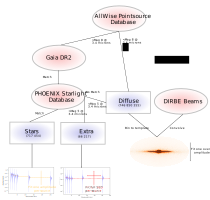
\includegraphics[width=\columnwidth]{figs/diagram/dirbe_diagram.pdf}\\
  \caption{Schematic diagram of the commander handling of compact objects in DIRBE. Red ovals are input data, and the blue boxes are the three classes of sources described in this paper. TODO: update bottom left image with final amplitude figure, update final number of sources to 424829, 710825587}
  \label{fig:diagram}
\end{figure}

\subsection{Stars}

\label{sec:starmodel}

We begin construction of the bright star model by taking the AllWise point source database \citep{wiseCat} and thresholding at Mag 7 in the W1 band. We then construct a unique sets of stars, starting with the brightest ones, which are no closer than 5 arcseconds to one another, which allows their parameters to be sampled without degeneracies. We repeat this procedure twice more, until we have three unique sampling groups of stars, all of which are far enough apart to be sampled simultaneously.

For each star in these groups we extract estimates of the effective temperature, $T_{\mathrm{eff}}$, the gravitational acceleration, $\log g$, and the metallicity, $[M/H]$, from the \GAIA\ DR2 database \citep{gaiaCat}, and use those to identify a best-fit spectral energy density (SED) from the PHOENIX starlight database \citep{Husser_2013}. The distributions of these parameters for the stars we select are shown in figure \ref{fig:gaiacat}. For stars with $T_{\mathrm{eff}} > 12000$K the PHOENIX catalog lacks data, which means that the 1.1\% of sources with higher temperatures use this 12000K temperature spectra as the closest match. This could lead to an issue with the SEDs of these hottest stars, but the overall amplitudes are fit per star which should mitigate the majority of this effect.

\begin{figure}
\includegraphics[width=\columnwidth]{figs/gaia/t_eff.pdf}
  \includegraphics[width=\columnwidth]{figs/gaia/logg.pdf}\\
  \includegraphics[width=\columnwidth]{figs/gaia/metalicity.pdf}\\
  \caption{Histograms of the three star parameters (effective temperature, gravity and metalicity) that are used by the PHOENIX database to determine the star SEDs, for the 424\ 829 stars used in this analysis.}
  \label{fig:gaiacat}
\end{figure}

The relationship between these stellar parameters and the star SEDs was examined in Figure \ref{fig:catalogueSEDs}. Although these effects are likely well known in the stellar astronomy community, we show them here for cosmologists (such as ourselves) who did not have an intuition for them. Here, we select a star with $T_{\mathrm{eff}}= 6000$K, $\log g = 3$ and $[M/H]= 0.0$ as our reference star. We then vary each of the three parameters slightly, holding the others constant and plot the two SEDs. The effective temperature is perhaps not surprisingly the dominant effect on the SED, especially when averaged over wide observing bands like those of DIRBE. A simpler model of star parameters in the far-infrared could perhaps neglect $\log g$ and $[M/H]$ entirely and produce SEDs based purely on $T_{\mathrm{eff}}$, and would be nearly as predictive, but we made a conservative choice to include all three parameters in the analysis regardless. 

\begin{figure}
\includegraphics[width=\columnwidth]{figs/gaia/star_SED_Teff.pdf}
\includegraphics[width=\columnwidth]{figs/gaia/star_SED_logg.pdf}
\includegraphics[width=\columnwidth]{figs/gaia/star_SED_MH.pdf}
  \caption{Comparison of PHOENIX spectra for different parameter compbinations. In each panel the black curve shows a reference star spectrum with $T_{\mathrm{eff}}= 6000$K, $\log g = 3.0$ and $[M/H]= 0.0$. The red curve shows, from top to bottom, the resulting spectra when setting $T_\mathrm{eff}=10\,000\,\mathrm{K}$, $\log g = 5.0$, and $[M/H]= -2.0$. The spectra shown in the middle panel have been smoothed to highlight the broad features that are mostly relevant for the current analysis.}
  \label{fig:catalogueSEDs}
\end{figure}

\begin{figure}
\includegraphics[width=\columnwidth]{figs/gaia/star_SED_logg_ratio_v2.pdf}
\caption{Ratio between the PHOENIX spectra shown in the middle panel of Fig.~\ref{fig:catalogueSEDs}, corresponding to $E(\log g = 5)/E(\log g  = 3)$. The vertical dashed lines indicate the positions of the six shortest wavelength DIRBE channels.}
  \label{fig:logg_ratio}
\end{figure}


The full Bayesian data model is shown in \cite{CG02_01}, and includes the bright star component $s_\mathrm{stars}(p, \lambda_j)$, the star emissions as a function of pixel $p$ and frequency $\lambda_j$ for a band $j$. Equation \ref{eq:datamodel} shows the data model for the star component that we describe in this paper:



\begin{equation}
 s_\mathrm{stars}(p, \lambda_j) = U_{\mathrm{mJy}} \sum_{j=1}^{n_{\mathrm{s}}}
  \epsilon_j(\nu)\,f_{\mathit{Gaia},j} a_{\mathrm{s},j}.
  \label{eq:datamodel}
\end{equation}

Here,$U_{\mathrm{mJy}}$ is a unit conversion factor, $a_{\mathrm{s},j}$ is the amplitude per source, $\epsilon_j(\nu)$ is the frequency dependent extinction factor and

\begin{equation}
f_{\mathit{Gaia}} = B_j(p, \lambda_j) E_j(\lambda_j),
\end{equation}

is the beam-convolved SED taken from the PHOENIX catalogue. 

Here, we sum over each star $j$, where $a_j$ is a single overall amplitude parameter fit per star and $B(p, \lambda)$ is the instrument beam for a detector at frequency $\lambda$ in a pixel $p$, centered on a source $j$. $E_i(\lambda)$ is the normalized emission for a given frequency $\lambda$. The emission $E_i$ is drawn directly from the \GAIA\ data and the PHOENIX starlight database, as discussed in section \ref{sec:phoenix}, and the beam $B$ is fixed for each detector. The extinction factor $\epsilon_j(\nu)$ is also just based on the existing \cite{ext_model} model, as detailed in section \ref{sec:extinction_model}, so we fit only the overall amplitude $a_i$ for each star in this model. This greatly reduces the degeneracies between the stars and other astrophysical components such as dust, and was found to work better than fitting a full SED per star. We include a star component in DIRBE bands 01--06 (1.25--25 $\mu$m), as at longer wavelengths the contribution from star emission was greatly subdominant to zodiacal light and dust, and including that data degraded the quality of the amplitude fits. 

To sample the star amplitudes $a_j$, we attempt to minimize the residual in each band for each source $j$, which can be expressed as a linear minimization problem, analogous to the mapmaking equation

\begin{equation}
\label{eq:minimize}
X_ja_j - Y_j = 0.
\end{equation}

where

\begin{equation}
X_j = S^T N^{-1} S = \sum_{i,p}\frac{E_{ij}^2 B^2_{ij}(p)}{\sigma_i^2(p)} 
\end{equation}

and

\begin{equation}
Y_j = S^TN^{-1}d = \sum_{i,p} \frac{E_{ij}B_{ij}(p) d_i(p)}{\sigma_i^2(p)}.
\end{equation}

Here, $\sigma_i^2(p)$ is the noise in pixel $p$ in band $i$, and $d_i(p)$ is the data map in band $i$ at pixel $p$. To reduce degeneracies, we fit the point sources on a data map with all other astrophysical components already removed, so $d_j(p)$ contains only noise and the point source $i$. The solution to \ref{eq:minimize} is simply $a_i = \frac{Y_j}{X_j}$, which gives a single overall amplitude for each star $j$. To sample the amplitudes, we also include a fluctuation term, such that our final proposal for the amplitudes is given by

\begin{equation}
a_i = \frac{Y_j}{X_j} + \frac{1}{\sqrt{X_j}} N_j(0,1),
\end{equation}

where $N_j(0,1)$ is a sample drawn from a unit Gaussian with 0 mean. 

\subsubsection{The PHOENIX Database}
\label{sec:phoenix}

To build the best SED model for each stellar source given the parameters retrieved from \GAIA, we do some post-processing of the spectra provided by the PHOENIX database to better match the measured values. PHOENIX provides spectra in finite resolution bins, as summarized in table \ref{tab:phoenix}, whereas the parameters estimated from the \GAIA\ data have arbitrary precision. Instead of simply selecting the closest spectrum to each star, we take a linear combination of the nearest 6 spectra, weighted by distance from the measured value, as given by 


\begin{align}
s &= \frac{1}{3}\bigg[\frac{s_{T-} (T_{+} - T) + s_{T+} (T - T_{-})}{T_{+} - T_{-}} \nonumber \\ 
&+ \frac{s_{g-} (g_{+} - g) + s_{g+} (g - g_{-})}{g_{+} - g_{-}} \nonumber \\
&+ \frac{s_{M-} (M_{+} - M) + s_{M+} (M - M_{-})}{M_{+} - M_{-}}\bigg].
\label{eq:starspec}
\end{align}

Here, $s$ is a spectra, and we have used $T$, $g$ and $M$ as short forms for $T_{\mathrm{eff}}$, $\log g$ and $[M/H]$. The subscripts + and - correspond to the closest reference value above and below the measured value (for example 0.0 and 0.5 if $\log g=$0.315). 

The second complicating factor is that the updated release of the catalogue\footnote{\href{https://www.astro.uni-jena.de/Users/theory/for2285-phoenix/grid.php}{\texttt{https://www.astro.uni-jena.de/Users/theory/\newline for2285-phoenix/grid.php}}} contains only a subset of the files in the original catalogue, although they are believed to be more accurate. This means that for stars in the extended parameter range, most importantly those with $\log g<$3.0, we must calculate their spectra using the older files. 

There, we run into the limitation that the older files are only defined to $\lambda=5.5\mu$m, compared to the newer files which go to $\lambda=50\mu$m. Amplitude estimates for these stars in the $12\mu$m and $25\mu$m bands must therefore be determined by first, computing the spectra with the old PHOENIX files and the new PHOENIX files, using the closest endpoint ($\log g$=3.0 in the most common case). Then, we compare the amplitudes in bands 3 and 4 ($3.5\mu$m and $4.9\mu$m), which gives us a ratio between the old spectra with the correct parameter range and the new spectra with the full wavelength coverage. Finally, we apply this scale factor to the points in bands 5 and 6 to obtain approximate amplitudes for those stars at longer wavelengths, based on the constant scaling shown in fig \ref{fig:logg_ratio}.

\begin{table}
    \centering
    \newcolumntype{C}{ @{}>{${}}r<{{}$}@{} }
    \begin{tabular}{l c c c c c }
    \hline
    \hline
     Param & Step Size & \multicolumn{2}{c}{Old} & \multicolumn{2}{c}{Updated}\\ 
     & & Min & Max & Min & Max\\
    \hline
    \hline
    $T_{\mathrm{eff}}$ (K) & 50-100K & 2300K & 12000K & 3000K & 11900K\\
    $\log g$ & 0.5 & 0.0 & 6.0 & 3.0 & 5.0 \\
    $[M/H]$ & 0.5 & -4.0 & 1.0 & -2.0 & 1.0 \\
     \hline
    \end{tabular}
    \caption{Parameters of spectra provided by the PHONEIX starlight database, both for the original and updated spectra.}
    \label{tab:phoenix}
\end{table}

\subsubsection{Binary Stars}

In the \Gaia\ database, 25\% of entries stronger than 12 mag were found to be binary stars. Whenever stars flagged as binaries in the \Gaia\ database also had estimated physical parameters, we first calculated the spectrum of each half of the binary according to Eq. \ref{eq:starspec}. Since the flux values are given per unit of area, we weighted the two spectra according to the estimated area of the corresponding star, so that the total flux estimated from the binary system
\begin{equation}
    s_{\mathrm{b}} = \frac{s_1 r_1^2+ s_2 r_2^2}{r_1^2 + r_2^2},
\end{equation}
where $s_{1, 2}$ and $r_{1, 2}$ denotes the flux and radius of the respective star in the binary system. The radii are not given explicitly in the \GAIA\ catalogue, so we use the estimate for the radius given in \cite{kuiper_1938}:
\begin{equation}
r = \exp\left(\frac{3.5\cdot 4}{5(3.5 \log(T_{\mathrm{eff}}) - \log(g))}\right ).
\end{equation}


\subsubsection{Extinction}
\label{sec:extinction_model}

At the highest frequencies, dust extinction $\epsilon(\nu)$ becomes one of the dominant effects on the star emission amplitudes, particularly in the galactic plane. We construct a simplified model of dust extinction, based on the work of \cite{ext_model} and \cite{fitzpatric_19}. We implement their 47 parameter model of dust extinction from the UV to the Infrared,\footnote{Note that we believe there is a typo in \cite{ext_model}, which has added an additional negative sign on their value of $b_{IR}\ \alpha_{1}$, and the correct value should be 1.06099} which provides a sky-averaged dust extinction parameter $\epsilon(\nu)$. 

We combine this spectral behaviour with with a full-sky spatial template using the $E(B-V)$ map from the Planck 2013 dataset \citep{planck_extinc_2013} by starting from Eq.~1 of \cite{ext_model}:

\begin{equation}
\frac{A(\lambda)}{A(V)} = a(\lambda) + b(\lambda)\left[ \frac{1}{R(V)} - \frac{1}{3.1}\right].
\end{equation}

Here, $\lambda$ is wavelength, $A$ is the absolute extinction, $a$ and $b$ are their model coefficients and $R(V)$ is given by

\begin{equation}
R(V) = \frac{A(V)}{E(B-V)},
\end{equation}

the ratio of absolute to selective extinction in the V band. Substituting this relationship in, and using the full sky average case of $R(V) =3.1$ \citep{fullsky_ext}, which allows us to omit the $b$ terms and obtain


\begin{equation}
A(\lambda) = 3.1\, E(B-V) a(\lambda).
\end{equation}

We then convert from the horrendous unit of magnitudes to a scaling factor that could actually be applied to our flux data, which gives an expression for the extinction ratio

\begin{equation}
\frac{F_{\mathrm{ext}}}{F_{\mathrm{raw}}} = \epsilon(\lambda) = e^{-\frac{3.1}{2.5} E(B-V) a(\lambda)}.
\end{equation}

The resulting spacial extinction template, evaluated in the 1.25$\mu$m band, can be seen in figure \ref{fig:ext_template}. The majority of the extinction is occurring in the galactic plane, but additional contributions can be seen tracing dust structures at high galactic latitudes. The template scales according to the relations shown in Figure 7 of \cite{ext_model}, and is applied to the stars component as described in eq. \ref{eq:datamodel}.

\begin{figure}
  \centering
  \includegraphics[width=\columnwidth]{figs/extinction/dirbe_extinction_1a.pdf}\\
  \caption{The full-sky extinction template used in this analysis, evaluated in the DIRBE 01 band at $1.25\mu$m.}
  \label{fig:ext_template}
\end{figure}

\subsection{Diffuse Star Emission}

\label{sec:diffusemodel}

Finally, after modelling the brightest sources using the method described above, we are left with a diffuse background of stars that are too dim to be individually resolved, but that in aggregate form a significant contribution to the total star signal at these wavelengths and so must be accounted for. We model this diffuse background using a single full-sky template, generated from the WISE W1 data at 3.4$\mu$m. We take the full AllWISE point source catalog, and select sources with a valid W1 magnitude that aren't already included in the bright point source model. We create a high resolution HEALpix \footnote{This is a footnote referring to the HEALPix website – currently \url{http://healpix.sourceforge.net}} map \citep{healpix} at nside=2048, and then add each source in turn to this map. We then downgrade the map to nside=512, which gives the map shown in Fig. \ref{fig:diffuse}. 

\begin{figure}
  \centering
  \includegraphics[width=\columnwidth]{figs/diffuseTemplate/diffuse_template.pdf}\\
  \caption{The unsmoothed template of diffuse star emission evaluated in the DIRBE 01 band, plotted on a log scale.}
  \label{fig:diffuse}
\end{figure}

\textit{This template is then included in the full sky model, with an amplitude fit jointly in bands 01-04, with an SED given by the mean of all SEDs of all the individual stars modelled in section \ref{sec:starmodel}. This SED is fit with a single amplitude parameter, which compensates for the overall difference in bandpass between W1 and the DIRBE bands. Although bands 5 and 6 do no contribute to the amplitude fit, the template is extrapolated to those bands as well and added to the total sky model.} MG: I think this is no longer true and that each band is fit independantly, but I wanted to confirm that with HK

\section{Astrophysical results}
\label{sec:results}

The model described in the previous section is then included in a full sky model, which includes galactic dust, zodical light and other components. A model of the DIRBE instrument is used to estimate other data artifacts, the most prominent of which was a sun-stationary signal of unknown origins. Following our previous work withing the Cosmoglobe framework \citep{BP01, watts2023_dr1}, we implement this model within the \texttt{commander3} codebase \citep{BP03}, which is our Bayesian end-to-end analysis pipeline. The full posterior of all our model parameters was then sampled using Gibbs sampling, exploring the full space around the maximum likelihood values of each parameter. We computed a total of NUMBER unique samples spread over 6 independent chains after discarding our burn-in data, which gave robust sample sizes for the results described here. 

In this paper, we present just the results of the star models described in section \ref{sec:models}, but we direct interested readers to the companion papers in the larger data release. More details on the overall sampling approach can be found in \citet{CG02_01}. The other components of the sky model are described in \citet{CG02_02}, \citet{CG02_05}, \citet{CG02_06} and \citet{CG02_07} and our limits on the CIB monopole derived from this work are presented in \citet{CG02_03}. 


\subsection{Maps}

In Figure \ref{fig:starsT} we show the mean star maps for the full pipeline run in all six DIRBE bands where they are modelled. Here, the maps show the sum of the star component and the diffuse background, which fully accounts for the point source emission over the full sky. As expected, the majority of the emission is found in the galactic plane, but there is also an important contribution from high latitude stars.

\begin{figure*}
  \centering
  \includegraphics[width=0.49\textwidth]{figs/starmaps/all_stars_mean_01.pdf}
  \includegraphics[width=0.49\textwidth]{figs/starmaps/all_stars_mean_02.pdf} \\
  \includegraphics[width=0.49\textwidth]{figs/starmaps/all_stars_mean_03.pdf}
  \includegraphics[width=0.49\textwidth]{figs/starmaps/all_stars_mean_04.pdf} \\
  \includegraphics[width=0.49\textwidth]{figs/starmaps/all_stars_mean_05.pdf}
  \includegraphics[width=0.49\textwidth]{figs/starmaps/all_stars_mean_06.pdf} \\
  \caption{Mean star maps from the Cosmoglobe DR2 release for the first 6 DIRBE bands. }
  \label{fig:starsT}
\end{figure*}

In Figure \ref{fig:zooms} we show zoom ins of a 20$^\mathrm{o}$ patch of sky centered at (lon, lat)= $20^\mathrm{o}, 70^\mathrm{o}$, plotting the DIRBE sky map in each band for the four highest frequency bands where the stars are most significant. In the second column, we show the total star model for the same region, then the resulting residual, and finally the overall chisq of the fit. The residuals contain a variety of mis-modeled point sources.

We can identify three types of point source residuals in this third column, although there are a large number of sources with residuals that are subdominant to the background noise level and so can be considered to be well modelled. Some of the point sources clearly show the imprints of spectral complexity, where the residual signature is blue in some bands and red in some others, which implies that our knowledge of the spectra is imperfect and a single overall amplitude fit was insufficient to model that source. The second class of residuals appear to be ring shapes, where the center of the point source is modelled well, but we oversubtract emission around the edges. This could be caused by our simplistic modelling of the DIRBE beams, which relies on the scanning strategy to symmeterize the otherwise square beam profile of the DIRBE instrument.

Other point source residuals are more complex, and look to be superpositions of multiple sources in the same region. These residuals could possibly be reduced by pruning point sources from the model that are too close to one another, or potentially by improving our models of the brightest sources. No attempt to do so was made in this work, as these residuals were only a small fraction of the total sky, and can be handled by masking using the chisq, which clearly shows these regions to be poorly modelled.

\begin{figure*}
  \includegraphics[width=0.95\textwidth]{figs/zoom/combined_zoom.pdf}\\
  \vspace{-8pt}
  \hspace{1.2in}
  \includegraphics[scale=0.7]{figs/zoom/cbar1.pdf}
  \hspace{0.95in}
  \includegraphics[scale=0.7]{figs/zoom/cbar2.pdf}
  \hspace{0.15in}
  \includegraphics[scale=0.7]{figs/zoom/cbar4_chisq.pdf}
  \caption{Zoom-ins on a subregion of the sky centred at $(20^\mathrm{o},70^\mathrm{o})$. The third column shows the difference between the two, and the final column is the overall chisq of the fit. TODO: update figure once chisq maps are done}
  \label{fig:zooms}
\end{figure*}


In Figure \ref{fig:amptrace}, we show the total amplitude of the stars in three pixels in different regions in the sky as a function of iteration, for all five of our  independent sampling chains. The first 25 samples in each chain are discarded as burn in, and the remaining samples (1090 in total) form the samples included our analysis. We see good mixing of the total amplitudes in the top row, although examining the individual components we do note that the full sky diffuse template mixes slower than the individual bright stars.

\begin{figure*}
  \centering
  \includegraphics[width=0.34\textwidth]{figs/mixing/trace_1352704.pdf}
  \includegraphics[width=0.31\textwidth]{figs/mixing/trace_2429499.pdf}
  \includegraphics[width=0.31\textwidth]{figs/mixing/trace_3121308.pdf}\\
  \caption{Trace plots of the total star amplitude in both chains for three pixels in different regions of the sky (low latitudes, the LMC and high latitudes) in DIRBE band 01. The dashed vertical line indicates the end of the burn in period, and samples after that are included in our final sample set.}
  \label{fig:amptrace}
\end{figure*}

\begin{figure*}
  \centering
  \includegraphics[width=\textwidth]{figs/correlation/covmatrix.pdf}
  \caption{Correlation plot showing a selection of parameters relevant for star modelling. From top to bottom: the monopoles for DIRBE channels 01-04, $N_{0}$ and $T_0$, the full sky ZL parameters, dust beta for the dust and cii correlated dust components, the amplitudes of three randomly selected stars, the diffuse template amplitude and the amplitudes and spectral indexes for two randomly selected extragalactic sources.}
  \label{fig:corr}
\end{figure*}

Figure \ref{fig:corr} shows the correlation matrix, computed between each parameter over all 1090 samples. In this case, we include a sample of star parameters, as well as some other parameters where we suspect degeneracies may occur. We see correlations between the monopoles of the 01, 02 and 03 bands, and anti correlations between some of the zodiacal light parameters, as has been studied in \citep{CG02_01, CG02_02}, but no correlations between these and the star model parameters, implying that they are independent.  We do not see much cross correlation between the star parameters and other parameters in the global chain, with the exception of the diffuse template and the zodiacal albedos ($A_{1,2,3}$) which show a mild anti-correlation. This implies that the star parameters are well mixed and are not degenerate with other full sky parameters in the run.

\subsection{Spectral Energy Densities}

In addition to the amplitude maps at each frequency, we can also examine the spectra energy densities (SEDs) of the sources within our model. Figure \ref{fig:starSEDs} shows the median SED model for all 424\ 829 star sources in our catalogue, as well as the SED for the diffuse template component. These follow a similar overall shape, although the diffuse stars fall off faster than the bright stars as we go to increasing wavelengths, perhaps due to selection effects between the two sets.

\begin{figure}
  \includegraphics[width=\columnwidth]{figs/starseds/star_seds.pdf}
  \caption{Star emission as a function of wavelength. The orange line is the median of all the individual stars fit in the model, with variances that are too small to see on this plot. The red curve is the mean of the diffuse template SED fit to the data, with the error bars showing the variance across the chain.}
  \label{fig:starSEDs}
\end{figure}

\subsection{Extinction}

We also investigate our model of extinction, to determine how well it approximated the real sky. WRITE SOMETHING HERE ONCE PLOT IS DONE \ref{fig:extinction}

\begin{figure}
\includegraphics[width=\columnwidth]{figs/diffuseTemplate/extinction.pdf}
  \caption{Profiles of the DIRBE Faint Star Model (FSM) and Cosmoglobe star model as a function of galactic latitude. A linear extrapolation is overplotted in the core region from -5 to 5 degrees galactic latitude, but excluding the galactic center from -1 to 1 degree. The theoretical value central value from this fit is compared to the measured values in the central bins to give estimates of the dust extinction in the galactic center for both cases. TODO:update once chisq is done}
  \label{fig:extinction}
\end{figure}

\textit{Figure \ref{fig:extinction} shows another comparison of these two models, highlighting mean behaviour as a function of galactic latitude which shows this missing extinction clearly. The DIRBE FSM shows clear dust extinction in the galactic center at 1.25 $\mu$m, as it explicitly incorporates extinction estimates from the 100 $\mu$m band, whereas the cosmoglobe model built from the \Gaia\ data does not show significant extinction on this plot. Regardless, it is surprising to not see any evidence of extinction in the galactic center as previous estimates such as \cite{extinction} estimate it at 70\% at 1 $\mu$m and 94\% at 3.4 $\mu$m. \emph{MG: Is this the case? I am confused by table 3 in rieke+lebofsky. Are they showing just the total scaling of the emissions, or is it actually a measure of the relative extinction in dusty regions?}}

\section{Comparison to other Analyses}
\label{sec:consistency}

\subsection{DIRBE FSM}

The original DIRBE analysis team \citep{dirbeFaint} also removed point sources from their measurement of the CIB emission, but followed a different approach. Instead of modelling the bright sources, the original analysis simply masked pixels brighter than a threshold (15 Jy in band 01), which resulted in cutting almost 35 \% of the sky at 1.25 $\mu$m. For the diffuse sources, they build a model (the ``faint source model'' or FSM) using the mechanism of \cite{wainscoat}, which integrates a model of source counts over the full sky, including models of galactic morphology, 87 discrete source types and the contribution from dust extinction. The results of this model in the DIRBE 01 band are shown in Figure \ref{fig:DIRBEfaint}, as well a comparison of the two models. 

The top two panels of Figure \ref{fig:DIRBEfaint} shows our diffuse template and the FSM, converted from QuadCube to HEALpix and plotted at nside=256. The third image shows the difference between these two templates of star emission, which clearly shows a difference in the treatment of dust extinction in the galactic plane. At 1.25$\mu$m, we can clearly see evidence of extinction in the DIRBE data, as can be seen in the fourth panel of Fig. \ref{fig:DIRBEfaint}, and so the fact that our model predicts none compared to the FSM is a clear shortcoming. 

\begin{figure}
\includegraphics[width=0.9\columnwidth]{figs/diffuseTemplate/diffuse_mean.pdf}  \vspace{-4pt}\\
  \includegraphics[width=0.9\columnwidth]{figs/diffuseTemplate/dirbe_template.pdf}\\
  \includegraphics[width=0.9\columnwidth]{figs/diffuseTemplate/diffuse_diff.pdf}\\
  %\includegraphics[width=0.9\columnwidth]{figs/diffuseTemplate/band_01_map.pdf}\\
  \includegraphics[width=0.9\columnwidth]{figs/diffuseTemplate/band01_res.pdf}\\
  \caption{The Commander diffuse star template (Top). Next: The DIRBE faint star model at 1.25 $\mu$m retrieved from LAMBDA and converted from QuadCube to healpix and the difference between that model and the diffuse template (position 3). The fourth panel shows our zodi-subtracted frequency map for the DIRBE 01 band, and the bottom panel shows the DIRBE 01 residual from the Commander run, indicating that our star model is slightly overestimating signal in the galactic plane, possibly due to missing extinction. TODO: update once chisq are done}
  \label{fig:DIRBEfaint}
\end{figure}

This difference shows that our model based on the integrated AllWISE point source catalogue predicts more star emission in the galactic plane than the DIRBE FSM in the inner part of the plane where dust extinction is dominant. This is likely due to the model being produced based on star emissions measured at 3.4$\mu$m, which shows less relative extinction than the data at 1.25$\mu$m. 

In the galactic bulge, our model predicts less emission than the FSM, which, when we look at the bottom panel of fig. \ref{fig:DIRBEfaint}, seems to be a better fit to the data. The blue residuals in the galactic center show that the model overpredicts emission in general in the galaxy, so  increasing the emission to the level that the FSM predicts would be a worse fit in this region. 



\subsection{DIRBE and 2MASS}

After the official DIRBE analysis, \cite{DIRBE2mass}, following \cite{gorjian} used the 2MASS catalogue to remove star emissions from DIRBE and find an improved upper limit on the CIB monopole, but were ultimately unable to claim a detection due to the zodiacal light contamination that they could not correct for. Their analysis looked at four dark patches of the sky and used 2MASS to estimate the contribution of both bright (K band magnitude > 14) and faint sources to the total signal in each patch, which we can compare with the Cosmoglobe estimates, as shown in Table \ref{tab:2mass}.

\begin{table*}
    \centering
    \newcolumntype{C}{ @{}>{${}}r<{{}$}@{} }
    \begin{tabular}{l c c c c c c c c c}
    \hline
    \hline
     Patch & $l$ & $b$ & $r$ & \multicolumn{2}{c}{Bright Stars} & \multicolumn{2}{c}{Diffuse Stars} & \multicolumn{2}{c}{Sum}\\ 
     & ($^{\circ}$) & ($^{\circ}$) & ($^{\circ}$) & \multicolumn{2}{c}{(kJy/sr)} & \multicolumn{2}{c}{(kJy/sr)} & \multicolumn{2}{c}{(kJy/sr)}\\
          &  & & & \cite{DIRBE2mass} & CG & \cite{DIRBE2mass} & CG  & \cite{DIRBE2mass} & CG\\
    \hline
    \hline
    \multicolumn{10}{c}{1.25$\mu$m}\\
    \hline
     1 \rule{0pt}{2ex} & 127.3 & 63.8 & 1.5 & 31.56 & 6.4 & 3.08 & 35.5 & 34.64 & 41.9\\
     2 & 107.7 & 57.7 & 2.0 & 42.72 & 9.2 & 3.62 & 44.5 & 45.34 & 53.7\\
     3 & 157.0 & -82.7 & 2.0 & 40.89 & 9.3 & 2.94 & 38.2 & 43.83 & 47.5\\
     4 & 257.8 & -59.4 & 1.9 & 51.88 & 14.2 & 3.92 & 44.4 & 55.8 & 58.6\\
     \hline
     \hline
     \multicolumn{10}{c}{2.2$\mu$m}\\
     \hline
     1 \rule{0pt}{2ex} & 127.3 & 63.8  & 1.5 & 20.79 & 4.4 & 1.58 & 23.1 & 22.37 & 27.5\\
     2 & 107.7 & 57.7 & 2.0 & 28.99 & 6.6 & 1.87 & 29.0 & 30.86 & 35.6\\
     3 & 157.0 & -82.7 & 2.0 & 28.62 & 7.0 & 1.50 & 24.8 & 30.12 & 31.8\\
     4 & 257.8 & -59.4 & 1.9 & 36.16 & 10.7 & 2.03 & 28.8 & 38.19 & 39.6\\
     \hline
    \end{tabular}
    \caption{Comparison of component intensities in patches from \cite{DIRBE2mass} and Cosmoglobe (CG) at 1.25 and 2.2 $\mu$m. The galactic longitude and latitude of the region center are given by $l$ and $b$, and $r$ is the radius of the field. The definitions of bright and diffuse sources differ between analyses, but the sum of the two allow reasonable comparison. TODO: update these numbers with new run}
    \label{tab:2mass}
\end{table*}


Differences in star classification between our analysis and \cite{DIRBE2mass} make it challenging to directly compare our amplitude estimates, but the sum of the bright and diffuse sources can still be compared. The Cosmoglobe analysis predicts about 20\% more total star emission, depending on the field and the frequency, which is probably due to having a much deeper star catalogue than 2MASS. By successfully modelling and removing more star emission, we are able to improve upon their limits on the CIB, as shown in \cite{CG02_03}. 

\section{Conclusions}
\label{sec:conclusions}

Stars are a critical component of the infrared sky, which must be correctly modelled in order to avoid contaminating other components. 

Figure \ref{fig:sed} shows the full sky average star SED derived from this work, plotted with the other sky signals as a function of frequency and wavelength, from the radio all the way to the infrared. The Cosmoglobe DR2 release, which this paper forms part of, is the first time a unified model of the sky has been shown to successfully describe all these frequencies, and the star model presented here is an integral part of this work.

\begin{figure*}
  \centering
  \includegraphics[width=\textwidth]{figs/sed/cg_spec_DR2_en.pdf}
  \caption{Components of the infrared temperature sky from 1$\mu$m to 1m wavelengths. The approximate contribution from stars is shown in yellow, and the observing bands from various experiments are indicated by the vertical lines. TODO: update with new run}
  \label{fig:sed}
\end{figure*}

\textit{Using the two classes of sources described in this paper, we were able to model 98\% of the observed DIRBE flux density at 1.25$\mu$m, dropping to 3\% at 25$\mu$m.} The star model showed robust mixing, and was able to fully describe the summed star emission in an effective manner. Our model was able to characterize and remove more star emission than previous works, which consequently was able to produce lower residuals and better constraints on the CIB monopoles, as discussed in the companion paper \citet{CG02_03}. Stars form the dominant foreground at these wavelengths, and so this model is an important contribution to the overall Cosmoglobe sky model, and can be re-used and adapted for future analyses using that framework.

\subsection{Future Work}

Including additional high frequency data directly in the the full run would be an important next step for this work, and will be the subject of future exploration in the collaboration. WISE is a major candidate experiment here, but also AKARI \citep{akari} and \IRAS\ \citep{neugebauer:1984} would be important complements to the work performed here. Incorporating these data directly could potentially give enough extra information to constrain the star SEDs directly instead of pre-computing them.

Additionally, the star model could be improved by the improving the dust extinction model. 

Another place within the model where there is room for improvement is in the treatment of the beams. Instead of assuming spherically symmerized beams, we could properly treat the unique square shape of the DIRBE response function, using techniques like deconvolution mapmaking \citep{artdeco}.

Finally, we could also improve our handling of the brightest stars, determining more accurate SEDs for those with $T_{\mathrm{eff}}>12000$K. This may help reduce the residuals around the brightest sources, and, combined with pruning the bright sources with 0 amplitudes could reduce the overall residual levels around these bright sources.


\begin{acknowledgements}
MG would like to thank Prof. Alberto Dominguez for useful conversations that led to improvements in the star modelling and better limits on the CIB monopoles at 1.25 $\mu$m.
 The current work has received funding from the European
  Union’s Horizon 2020 research and innovation programme under grant
  agreement numbers 819478 (ERC; \textsc{Cosmoglobe}) and 772253 (ERC;
  \textsc{bits2cosmology}). Some of the results in this paper have been derived using the HEALPix \citep{healpix} package.
  We acknowledge the use of the Legacy Archive for Microwave Background Data
  Analysis (LAMBDA), part of the High Energy Astrophysics Science Archive Center
  (HEASARC). HEASARC/LAMBDA is a service of the Astrophysics Science Division at
  the NASA Goddard Space Flight Center.  
  
   This publication makes use of data products from the Wide-field Infrared Survey Explorer, which is a joint project of the University of California, Los Angeles, and the Jet Propulsion Laboratory/California Institute of Technology, and NEOWISE, which is a project of the Jet Propulsion Laboratory/California Institute of Technology. WISE and NEOWISE are funded by the National Aeronautics and Space Administration.
   
   This work has made use of data from the European Space Agency (ESA) mission
{\it Gaia} (\url{https://www.cosmos.esa.int/gaia}), processed by the {\it Gaia}
Data Processing and Analysis Consortium (DPAC,
\url{https://www.cosmos.esa.int/web/gaia/dpac/consortium}). Funding for the DPAC
has been provided by national institutions, in particular the institutions
participating in the {\it Gaia} Multilateral Agreement.
\end{acknowledgements}


%-------------------------------------------------------------
%                                       Table with references 
%-------------------------------------------------------------
%

\bibliographystyle{aa}
\bibliography{references, ../../common/CG_bibliography}
\end{document}
%%%% End of aa.dem


